\documentclass[a4paper,12px]{article}
\usepackage{graphicx}
\usepackage[english]{babel}
\usepackage{fullpage}
\usepackage{xfrac}
\usepackage{fancyhdr}
\usepackage{lastpage}
\usepackage{xifthen}
\usepackage[linesnumberedhidden, titlenotnumbered]{algorithm2e}
\usepackage{lipsum}
\usepackage{hyperref}
\usepackage{array}
\usepackage{tabularx}
\usepackage{caption}
\usepackage{amsfonts}
\usepackage{amssymb}
\usepackage{amsmath}
\usepackage{mathtools}
\usepackage{placeins}
\usepackage{enumitem}
\usepackage[noabbrev]{cleveref}
\usepackage[utf8]{inputenc}
\usepackage{multirow}

\usepackage{minted}
\usepackage{listings}
\usepackage{dsfont}
\usepackage{units}

\pagestyle{fancy}
\lhead{\includegraphics[width=7cm]{logoUvA}}
\rhead{\footnotesize \textsc {Report\\ \opdracht}}
\lfoot%
{%
    \footnotesize \studentA%
    \ifthenelse{\isundefined{\studentB}}{}{\\ \studentB}
    \ifthenelse{\isundefined{\studentC}}{}{\\ \studentC}
    \ifthenelse{\isundefined{\studentD}}{}{\\ \studentD}
    \ifthenelse{\isundefined{\studentE}}{}{\\ \studentE}
}
\cfoot{}
\rfoot{\small \textsc {Page \thepage\ of~\pageref{LastPage}}}
\renewcommand{\footrulewidth}{0.5pt}

\fancypagestyle{firststyle}
{%
    \fancyhf{}
    \renewcommand{\headrulewidth}{0pt}
    \chead{\includegraphics[width=7cm]{logoUvA}}
    \rfoot{\small \textsc {Page \thepage\ of~\pageref{LastPage}}}
}

\setlength{\topmargin}{-0.3in}
\setlength{\textheight}{630pt}
\setlength{\headsep}{40pt}
\setlength{\parindent}{0pt}

% =================================== DOC INFO ===================================

\newcommand{\opdracht}{Theoretical Excercises}
\newcommand{\titel}{Labs week 3}
\newcommand{\docent}{Alban Ponse, Bob Diertens}
\newcommand{\cursus}{Theoretische aspecten van de Programmatuur}
\newcommand{\vakcode}{}
\newcommand{\datum}{\today}
\newcommand{\studentA}{Maico Timmerman}
\newcommand{\uvanetidA}{10542590}
%\newcommand{\studentB}{Tim van Zalingen}
\newcommand{\uvanetidB}{10784012}
% \newcommand{\studentC}{Boudewijn Braams}
\newcommand{\uvanetidC}{10401040}
% \newcommand{\studentD}{Govert Verkes}
\newcommand{\uvanetidD}{10211748}
%\newcommand{\studentE}{Naam student 5}
\newcommand{\uvanetidE}{UvAnetID student 5}

% ===================================  ===================================

\begin{document}
\thispagestyle{firststyle}
\begin{center}
    \textsc{\Large \opdracht}\\[0.2cm]
    \rule{\linewidth}{0.5pt} \\[0.4cm]
    {\huge \bfseries \titel}
    \rule{\linewidth}{0.5pt} \\[0.2cm]
    {\large \datum\\[0.4cm]}

    \begin{minipage}{0.4\textwidth}
        \begin{flushleft}

            \emph{Student:}\\
            {\studentA\\ {\small \uvanetidA\\[0.2cm]}}
            \ifthenelse{\isundefined{\studentB}}{}{\studentB\\ {\small \uvanetidB\\[0.2cm]}}
        \end{flushleft}
    \end{minipage}~%
    \begin{minipage}{0.4\textwidth}
        \begin{flushright}
            \emph{Lecturers:} \\
            \docent\\[0.2cm]
            \emph{Course:} \\
            \cursus\\[0.2cm]
            % \emph{Student:}\\
            \ifthenelse{\isundefined{\studentC}}{}{\studentC\\ {\small \uvanetidC\\[0.2cm]}}
            \ifthenelse{\isundefined{\studentD}}{}{\studentD\\ {\small \uvanetidD\\[0.2cm]}}
            \ifthenelse{\isundefined{\studentE}}{}{\studentE\\ {\small \uvanetidE\\ [0.2cm]}}
        \end{flushright}
    \end{minipage}\\[1 cm]
\end{center}


% =================================== CONTENTS ===================================

% \tableofcontents

\newcommand{\Sum}[2]{\sum^{#2}_{#1}}
\newcommand{\E}[1]{{\mathbb{E}\left[#1\right]}}
\newcommand{\var}[1]{{\text{var}\left[#1\right]}}
\newcommand{\diffpart}[1]{\frac{\partial}{\partial{} #1}}
\newcommand{\?}{\stackrel{?}{=}}
\newcommand{\intinf}{\int\limits_{-\infty}^{\infty}}
\newcommand{\intnulinf}{\int\limits_{0}^{\infty}}
\newcommand{\intpi}{\int\limits_{0}^{2\pi}}
\newcommand{\argmin}[1]{\underset{#1}{\mathop{\mathrm{argmin}}}}
\newcommand{\argmax}[1]{\underset{#1}{\mathop{\mathrm{argmax}}}}
\definecolor{bg}{rgb}{0.95,0.95,0.95}
% =================================== MAIN TEXT ===================================


\section{Factory}

\subsection{3.2.1 Opdracht 1}

\begin{figure}[h]
    \centering
    \includegraphics[width=\linewidth]{without_lock.png}
    \caption{Factory for which locking is unneccesary.}
    \label{fig:without_lock}
\end{figure}
\FloatBarrier%

The initial factory seen in \autoref{fig:without_lock} is a factory that does
not require any form of locking. Writing to the channel is done twice, first
filling the channel with a value and afterwards emptying the channel (writing
empty). The working cells can never reach a situation in which they
overwrite/remove a value before it is read. They check if the channel is
empty/filled and act accordingly with an atomic action. Thus in a single cycle,
the value is changed. For reading of the value it actually takes 2 cycles,
however the value in the channel is only removed after it has been loaded to
the working cell. The working cell at the other end of the channel will never
act, since there is still a value in the channel.

An example of a working cell reading a value of a channel and outputting to the
output queue is displayed in the code below. \footnote{Implementation in:
factory\_without\_lock.msp.thr}

\begin{minted}[bgcolor=bg]{C}
// Label to reference the entry point of the code for this thread.
L2;
// Test if the working cell is empty.
+wc2.v==""{;
    // Cell is empty, test if a value can be fetched.
    +channel12.v==""{;
        // Channel is also empty, do nothing.
    }{;
        // Channel has values, thus fetch it into the working cell.
        first channel12.v wc2.v;
        delfirst channel12.v;
    };
    // Restart the thread.
    ##L2;
}{;
    // Cell has a value, thus write to output.
    append output.q wc2.v;
    delfirst wc2.v;
    ##L2;
};
\end{minted}

\subsection{3.2.2 Opdracht 2}

\begin{figure}[h]
    \centering
    \includegraphics[width=\linewidth]{factory.png}
    \caption{Fluid of factory using 3 working cells and 2 instances of wc2.}
    \label{fig:factory}
\end{figure}
\FloatBarrier%
The fluid of the factory after adding an additional working cell 2 can be seen in \autoref{fig:factory}.

Since both working cell 2's use the \verb|channel12|, atomic operations are
need to make sure both the cells do not read the same value to process of the
channel. For this problem a locking system has been introduced. The instruction
for field introduction is atomic and returns \verb|true| or \verb|false|
depending on success. By executing this instruction as a test-instruction, locks
can be placed on the channel and working cells can act accordingly. If the lock
is set successfully, the cell takes the value and empties the channel. If not,
it will retry the next instruction.

An example of the implementation of the code for working cell 2 is displayed below. An \verb|a| or \verb|b| is appended to the name for referencing the correct foci. \footnote{Implementation in: factory\_with\_lock.msp.thr}

\begin{minted}[bgcolor=bg]{C}
// Label to reference the entry point of the code for this thread.
L22;
// Test if the working cell is empty.
+wc2b.v==""{;
    // Test if the channel has a value, if not, restart thread.
    +channel12.v==""; ##L22;
    // Channel has a value, thus try to lock, if fails, restart thread.
    -channel12.+lock; ##L22;
    // Double check if the value has not been taken yet by another thread.
    +channel12.v==""{;
        // Value is already taken.
    }{;
        // Process value by taking from channel and placing in working cell.
        first channel12.v wc2b.v;
        // Removed channels value.
        delfirst channel12.v;
    };
    // Unlock and restart thread.
    channel12.-lock;
    ##L22;
}{;
    // Cell has a value, thus write to output.
    append output.q wc2b.v;
    delfirst wc2b.v;
    ##L22;
};
\end{minted}

An example of the lock in action can be seen in \autoref{fig:lock_in_action}.
\begin{figure}[h]
    \centering
    \includegraphics[width=\linewidth]{lock_in_action.png}
    \caption{Lock placed on channel12, to prevent other wc2's of accessing it.}
    \label{fig:lock_in_action}
\end{figure}
\FloatBarrier%

\subsection{4.1.1 Opdracht 1}

\begin{figure}[h]
    \centering
    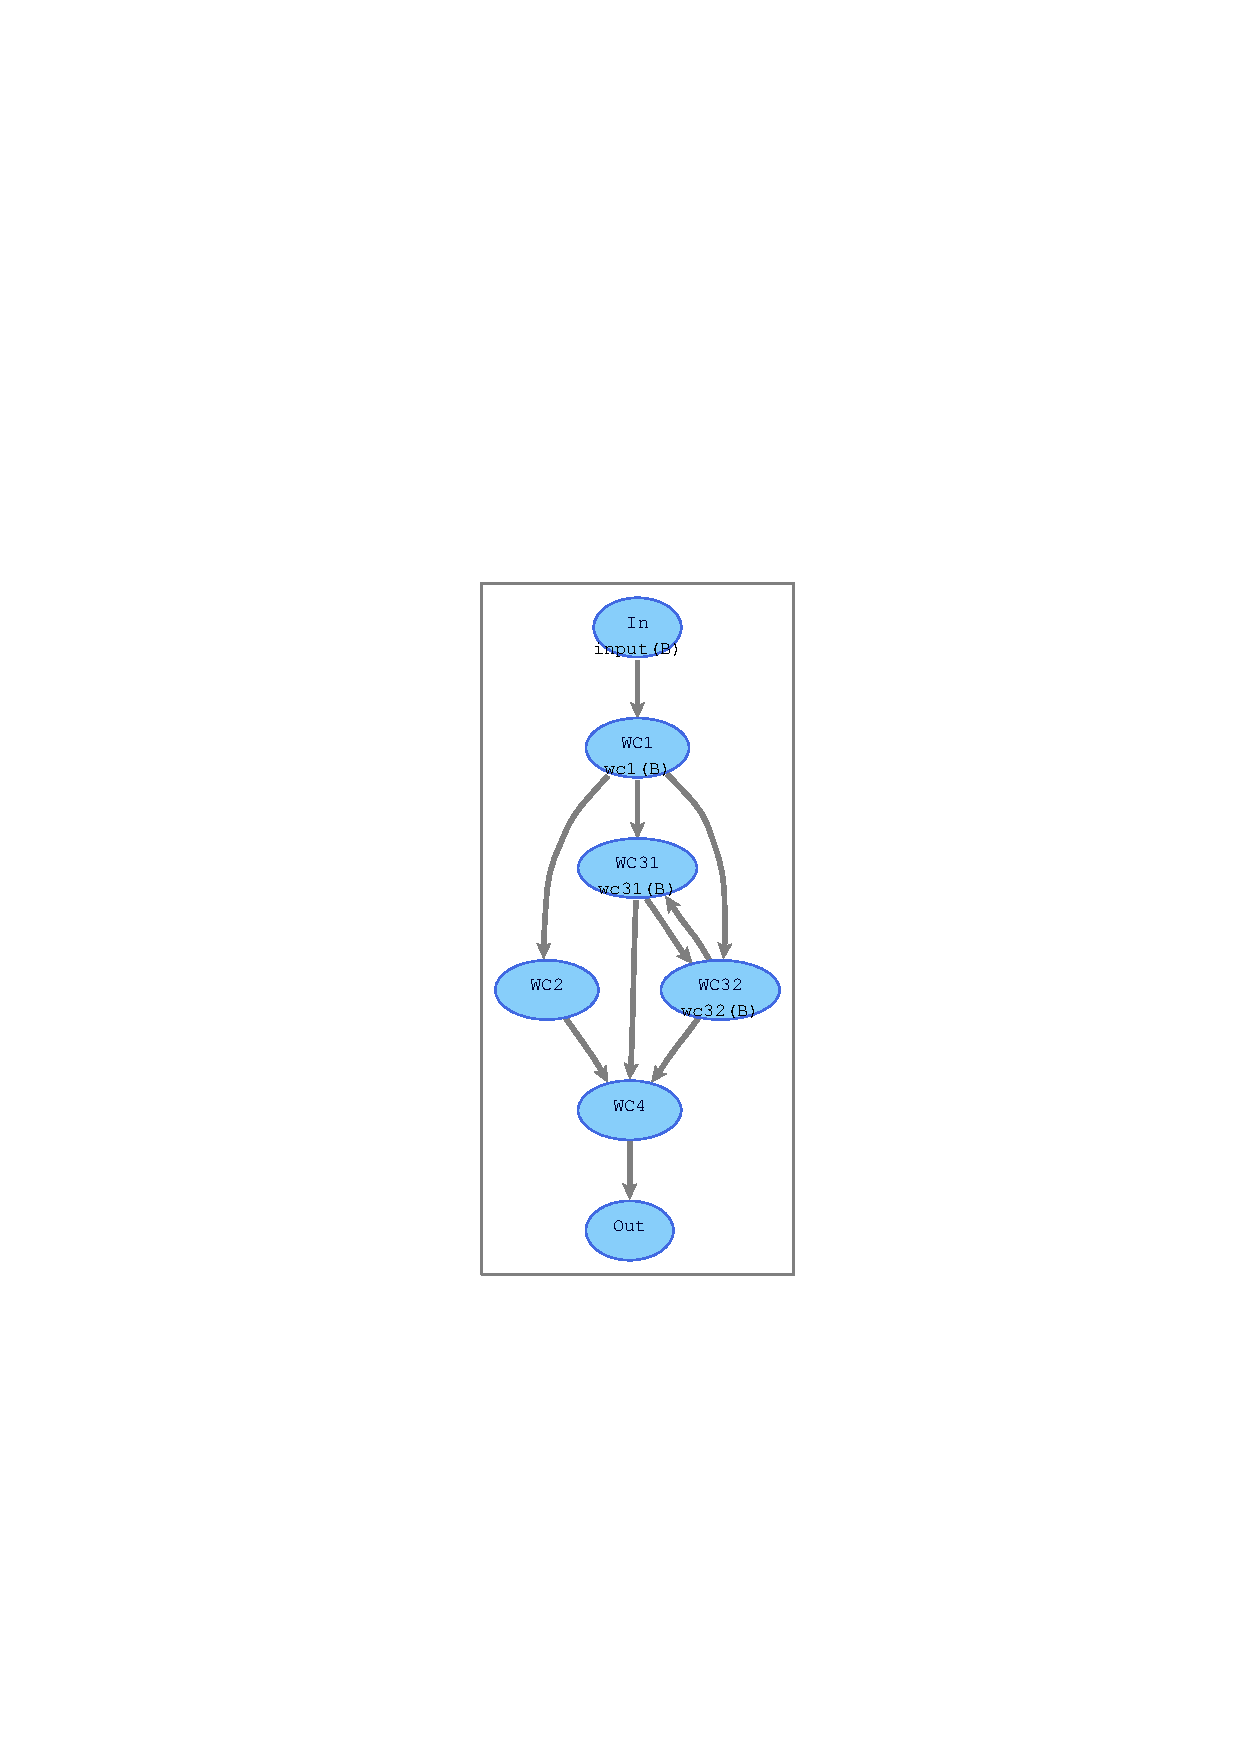
\includegraphics[width=\linewidth]{deadlock.png}
    \caption{Deadlock between wc2 and wc3. Both channels and working cells filled.}
    \label{fig:deadlock}
\end{figure}
\FloatBarrier%

In the new factory products can flow between working cell 2 and 3 in both
directions. This can cause deadlock, as can been seen \autoref{fig:deadlock}.
In this example figure the requirement for deadlock can be seen. Both channels
are filled with their products and the working cells hold products, which need
to input into the channels. However for the product to be placed in the
channel, the channel needs to be emptied by the other working cell. Since both
working cells suffer this problem, a situation of deadlock is created. Neither
of the cells can do anything.

\subsection{4.1.2 Opdracht 2}

By changing the channels from single product to multiple product buffers, the
deadlock is solved .\footnote{Implementation in:
factory\_channel\_buffer.msp.thr} A working cell is always able to place its
product into the

channel, after which it can take the first value of the channel. Since there
are no working cells which use the same channel on the same side, locking is
not needed here.

In theory this solution will always work, however, when a single working cell
taking output cannot keep up with the input, the system can still fail. In
theory channels can have infinitely large buffers, however in practice, there
are limits. This means that there is a option of buffer-overflow.

% =================================== REFERENCES ===================================

% \clearpage

% \bibliographystyle{apalike}
% \bibliography{report}

\end{document}
